%%
%% This file is based on `sample-manuscript.tex' from acmart-primary package
%%
%%
%% Commands for TeXCount
%TC:macro \cite [option:text,text]
%TC:macro \citep [option:text,text]
%TC:macro \citet [option:text,text]
%TC:envir table 0 1
%TC:envir table* 0 1
%TC:envir tabular [ignore] word
%TC:envir displaymath 0 word
%TC:envir math 0 word
%TC:envir comment 0 0
%%
%%
%% The first command in your LaTeX source must be the \documentclass command.
%%\documentclass[manuscript,screen,review]{acmart}
\documentclass[manuscript,review]{acmart}

%%
%% \BibTeX command to typeset BibTeX logo in the docs
\AtBeginDocument{%
  \providecommand\BibTeX{{%
    Bib\TeX}}}

%% Rights management information.  This information is sent to you
%% when you complete the rights form.  These commands have SAMPLE
%% values in them; it is your responsibility as an author to replace
%% the commands and values with those provided to you when you
%% complete the rights form.
\setcopyright{acmcopyright}
\copyrightyear{2022}
\acmYear{2022}
\acmDOI{XXXXXXX.XXXXXXX}

%% These commands are for a PROCEEDINGS abstract or paper.
\acmConference[Conference acronym 'XX]{Make sure to enter the correct
  conference title from your rights confirmation emai}{June 03--05,
  2018}{Woodstock, NY}
\acmPrice{15.00}
\acmISBN{978-1-4503-XXXX-X/18/06}


%%
%% Submission ID.
%% Use this when submitting an article to a sponsored event. You'll
%% receive a unique submission ID from the organizers
%% of the event, and this ID should be used as the parameter to this command.
%%\acmSubmissionID{123-A56-BU3}

%%
%% For managing citations, it is recommended to use bibliography
%% files in BibTeX format.
%%
%% You can then either use BibTeX with the ACM-Reference-Format style,
%% or BibLaTeX with the acmnumeric or acmauthoryear sytles, that include
%% support for advanced citation of software artefact from the
%% biblatex-software package, also separately available on CTAN.
%%
%% Look at the sample-*-biblatex.tex files for templates showcasing
%% the biblatex styles.
%%

%%
%% The majority of ACM publications use numbered citations and
%% references.  The command \citestyle{authoryear} switches to the
%% "author year" style.
%%
%% If you are preparing content for an event
%% sponsored by ACM SIGGRAPH, you must use the "author year" style of
%% citations and references.
%% Uncommenting
%% the next command will enable that style.
%%\citestyle{acmauthoryear}



%%%%%%%%%%%%%%%%%%%%%%%%%%%%%%%%%%%%%%%%%%%%%%%%%%%%%%



%%
%% end of the preamble, start of the body of the document source.
\begin{document}

%%
%% The "title" command has an optional parameter,
%% allowing the author to define a "short title" to be used in page headers.
\title{"Hey Oktavia!": A Case Study on Voice User Interface Design for Piano Practice}

%%
%% The "author" command and its associated commands are used to define
%% the authors and their affiliations.
%% Of note is the shared affiliation of the first two authors, and the
%% "authornote" and "authornotemark" commands
%% used to denote shared contribution to the research.
\author{Julia Honeder}
\email{julia.honeder@students.fh-ooe.at}
\author{Kathrin Probst}
\email{kathrin.probst@fh-ooe.at}
\affiliation{%
  \institution{University of Applied Sciences Upper Austria}
  \city{Hagenberg}
  \country{Austria}
}


%%
%% By default, the full list of authors will be used in the page
%% headers. Often, this list is too long, and will overlap
%% other information printed in the page headers. This command allows
%% the author to define a more concise list
%% of authors' names for this purpose.

%%\renewcommand{\shortauthors}{Trovato et al.}


%%
%% The abstract is a short summary of the work to be presented in the
%% article.
\begin{abstract}
Abstract.
\end{abstract}


%%
%% The code below is generated by the tool at http://dl.acm.org/ccs.cfm.
%% Please copy and paste the code instead of the example below.
%%
\begin{CCSXML}
<ccs2012>

<concept>
<concept_id>10003120.10003123.10011759</concept_id>
<concept_desc>Human-centered computing~Empirical studies in interaction design</concept_desc>
<concept_significance>500</concept_significance>
</concept>

<concept>
<concept_id>10003120.10003121.10003124.10010870</concept_id>
<concept_desc>Human-centered computing~Natural language interfaces</concept_desc>
<concept_significance>500</concept_significance>
</concept>

</ccs2012>
\end{CCSXML}

\ccsdesc[500]{Human-centered computing~Empirical studies in interaction design}
\ccsdesc[500]{Human-centered computing~Natural language interfaces}


%%
%% Keywords. The author(s) should pick words that accurately describe
%% the work being presented. Separate the keywords with commas.
\keywords{voice interaction, conversational interfaces, musical instruments, piano}

%%
%% This command processes the author and affiliation and title
%% information and builds the first part of the formatted document.
\maketitle




%%%%%%%%%%%%%%%%%%%%%%%%%%%%%%%%%%%%%%%%%%%%%%%%%%%%%%




\section{Introduction}
Introduction \cite{Cohen04}.

\begin{figure}[h]
  \centering
  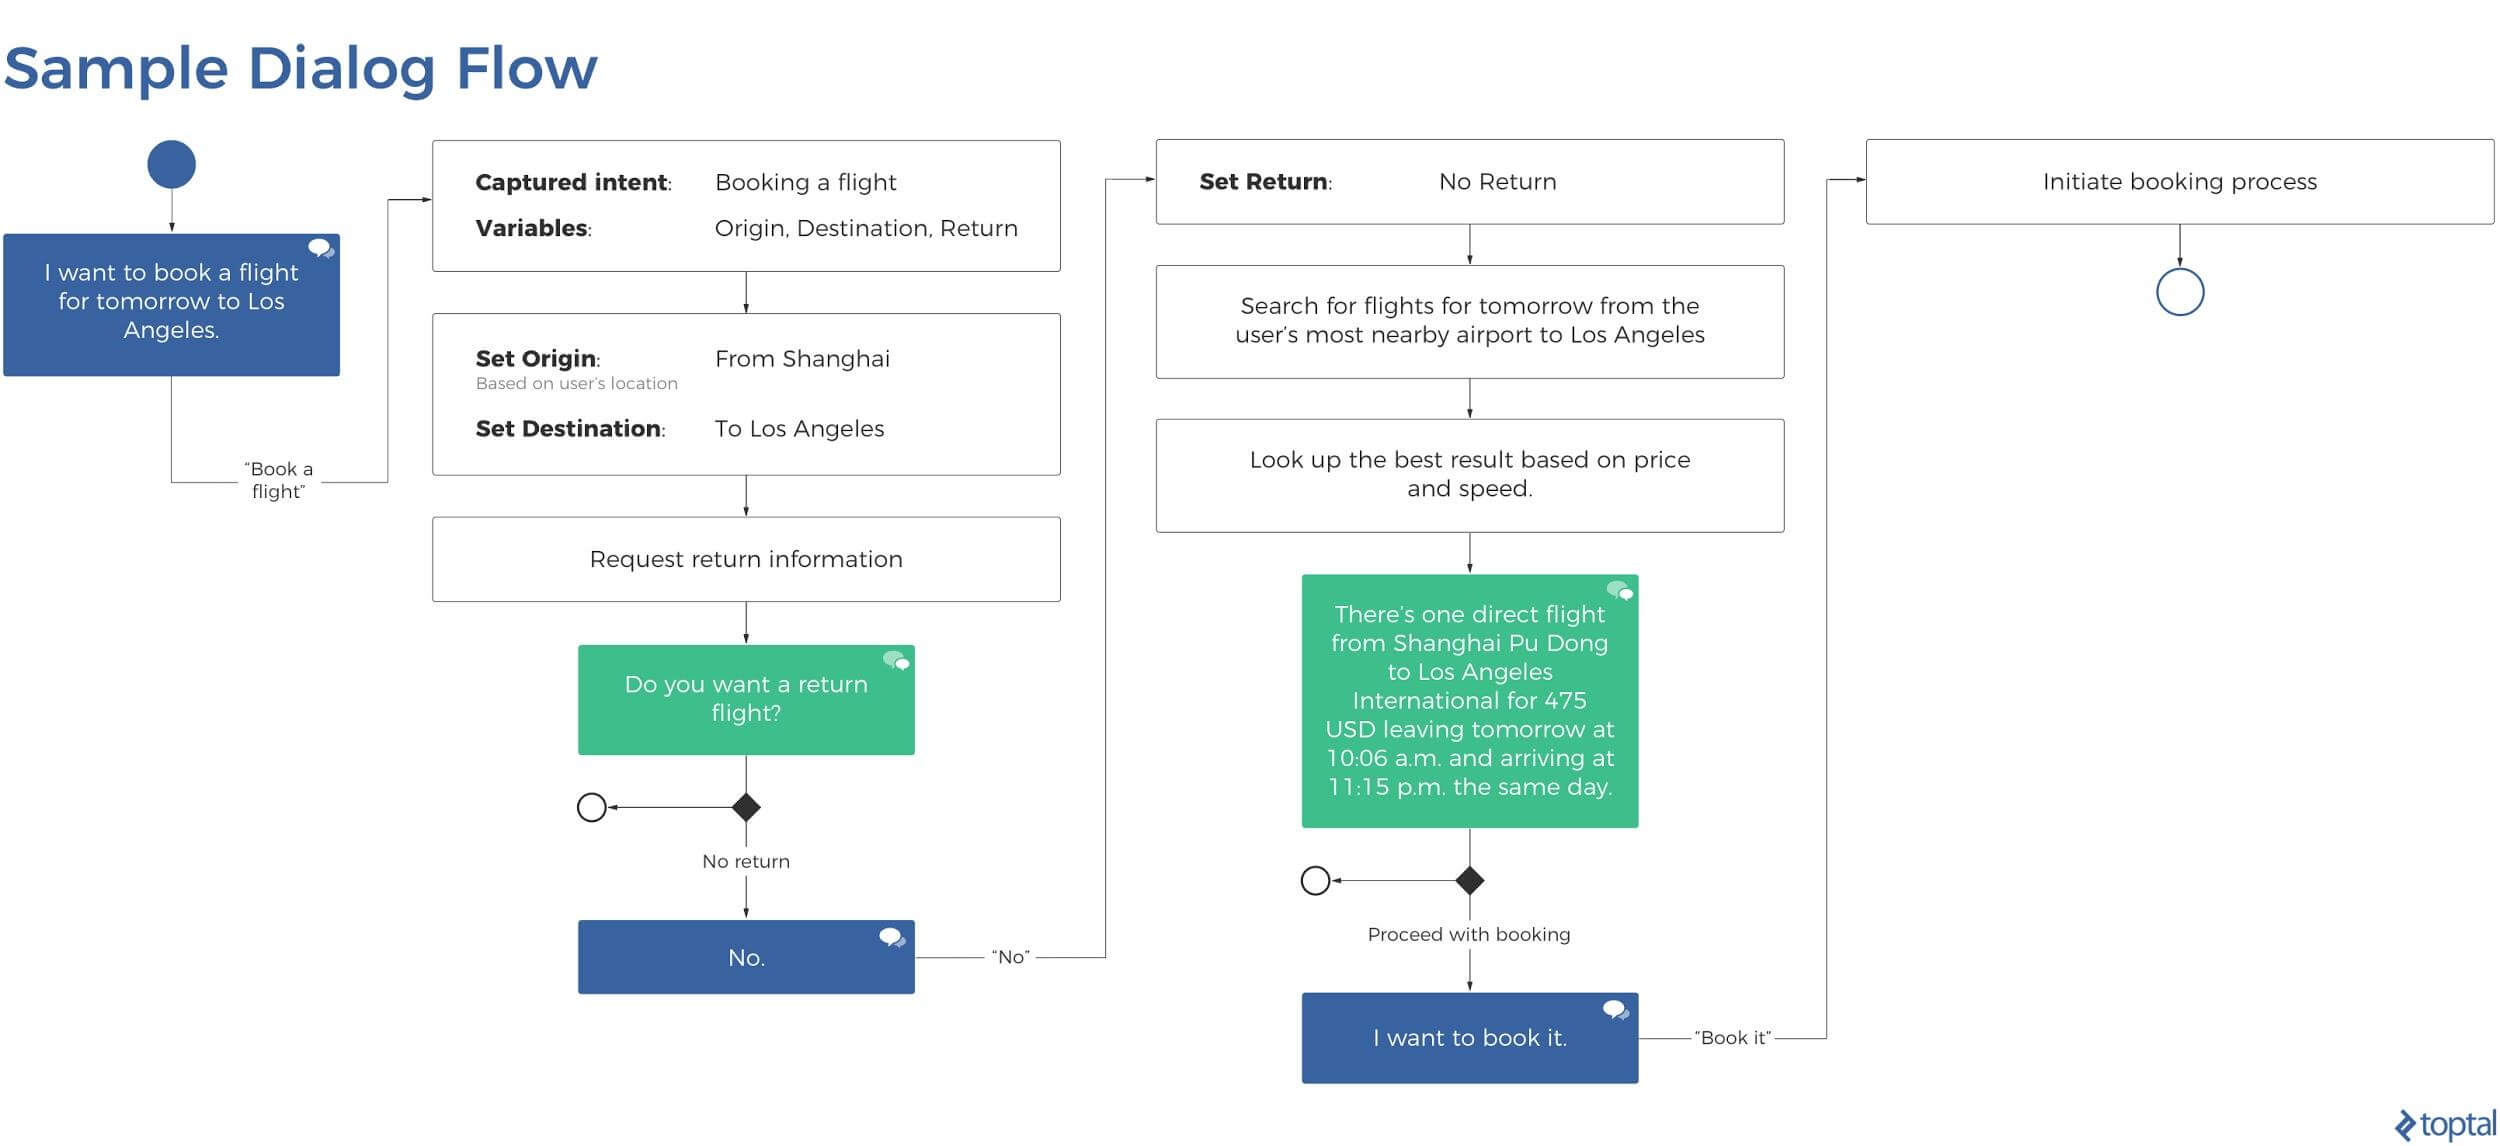
\includegraphics[width=\linewidth]{images/sample}
  \caption{Caption.}
  \Description{Description.}
\end{figure}

%% Related Work is not necessary for CHI Case Studies
%%\section{Related Work}


\section{Design Process}
Design Process.


\section{Study Design and Data Collection}
Evaluation.


\section{Reflection}
Reflection.


\section{Conclusion}
Conclusion.




%%%%%%%%%%%%%%%%%%%%%%%%%%%%%%%%%%%%%%%%%%%%%%%%%%%%%%





%%
%% The acknowledgments section is defined using the "acks" environment
%% (and NOT an unnumbered section). This ensures the proper
%% identification of the section in the article metadata, and the
%% consistent spelling of the heading.
\begin{acks}
To Robert, for the bagels and explaining CMYK and color spaces.
\end{acks}

%%
%% The next two lines define the bibliography style to be used, and
%% the bibliography file.
\bibliographystyle{ACM-Reference-Format}
\bibliography{references}





%%%%%%%%%%%%%%%%%%%%%%%%%%%%%%%%%%%%%%%%%%%%%%%%%%%%%%




%%
%% If your work has an appendix, this is the place to put it.
\appendix

\section{Wizard-of-Oz Prototypes}



\end{document}
\endinput
%%
%% End of file `sample-manuscript.tex'.
